%%%%%%%%%%%%%%%%%%%%%%%%%%%%%%%%%%%%%%%%%
% Presentación Beamer - Plantilla en LaTeX
% Versión 2.0 (8 de marzo de 2022)
% Plantilla original: https://www.LaTeXTemplates.com
% Autor: Vel (vel@latextemplates.com)
% Licencia: CC BY-NC-SA 4.0
%%%%%%%%%%%%%%%%%%%%%%%%%%%%%%%%%%%%%%%%%

%%%%%%%%%%%%%%%%%%%%%%%%%%%%%%%%%%%%%%%%%
% Este modelo de presentación fue 
% creado a partir del modelo de Giovanni Spadaro.
% Disponible en: 
% https://github.com/Giovo17/presentation-template-unict-lm-data
%
% Adaptado por Lucas Amaral Taylor para crear una versión especial 
% para los estudiantes de Matemáticas y Estadística de la USP (IME-USP).
% Disponible en:
% https://github.com/lucasamtaylor01/IME-template
%%%%%%%%%%%%%%%%%%%%%%%%%%%%%%%%%%%%%%%%%

\documentclass[
	11pt, % Tamaño de fuente predeterminado
	% t, % Alineación vertical superior
	%aspectratio=169, % Definir proporción 16:9
]{beamer}

% Ruta de las imágenes
\graphicspath{{img/}}

% Paquetes adicionales
\usepackage[spanish]{babel}
\usepackage[alf]{abntex2cite} % Citas ABNT
\usepackage{booktabs} % Mejoras en las líneas de tablas
\usepackage{palatino} % Fuente Palatino
\usepackage[default]{opensans} % Fuente Open Sans
\usepackage{subcaption}
%----------------------------------------------------------------------------------------
%	PACOTES E CONFIGURAÇÕES PARA CÓDIGO
%----------------------------------------------------------------------------------------
% Pacotes necessários para formatação de código
\usepackage[utf8]{inputenc}
\usepackage{listings}
\usepackage{xcolor}

% Cores para syntax highlighting (VSCode Light Theme)
\definecolor{vscBackground}{RGB}{255,255,255}    % Fundo branco
\definecolor{vscKeyword}{RGB}{175,0,219}         % Roxo para palavras-chave
\definecolor{vscString}{RGB}{163,21,21}          % Vermelho para strings
\definecolor{vscComment}{RGB}{0,128,0}           % Verde para comentários
\definecolor{vscFunction}{RGB}{121,94,38}        % Marrom para funções
\definecolor{vscNumber}{RGB}{9,134,88}           % Verde escuro para números
\definecolor{vscOperator}{RGB}{175,0,219}        % Roxo para operadores
\definecolor{vscText}{RGB}{0,0,0}                % Texto preto
\definecolor{vscLineNr}{RGB}{128,128,128}        % Cinza para números de linha

% Configuração geral do listings para UTF-8
\lstset{
    inputencoding=utf8,
    extendedchars=true,
    literate=%
        {á}{{\'a}}1 {é}{{\'e}}1 {í}{{\'i}}1 {ó}{{\'o}}1 {ú}{{\'u}}1
        {Á}{{\'A}}1 {É}{{\'E}}1 {Í}{{\'I}}1 {Ó}{{\'O}}1 {Ú}{{\'U}}1
        {à}{{\`a}}1 {è}{{\`e}}1 {ì}{{\`i}}1 {ò}{{\`o}}1 {ù}{{\`u}}1
        {À}{{\`A}}1 {È}{{\'E}}1 {Ì}{{\`I}}1 {Ò}{{\`O}}1 {Ù}{{\`U}}1
        {ã}{{\~a}}1 {ẽ}{{\~e}}1 {ĩ}{{\~i}}1 {õ}{{\~o}}1 {ũ}{{\~u}}1
        {Ã}{{\~A}}1 {Ẽ}{{\~E}}1 {Ĩ}{{\~I}}1 {Õ}{{\~O}}1 {Ũ}{{\~U}}1
        {â}{{\^a}}1 {ê}{{\^e}}1 {î}{{\^i}}1 {ô}{{\^o}}1 {û}{{\^u}}1
        {Â}{{\^A}}1 {Ê}{{\^E}}1 {Î}{{\^I}}1 {Ô}{{\^O}}1 {Û}{{\^U}}1
        {ç}{{\c c}}1 {Ç}{{\c C}}1
        {º}{{\textordmasculine}}1
        {ª}{{\textordfeminine}}1
}

% Configurações base comum para todas as linguagens
\lstdefinestyle{baseStyle}{
    backgroundcolor=\color{vscBackground},
    basicstyle=\ttfamily\small\color{vscText},
    breakatwhitespace=false,
    breaklines=true,
    captionpos=b,
    keepspaces=true,
    numbers=left,
    numbersep=5pt,
    showspaces=false,
    showstringspaces=false,
    showtabs=false,
    tabsize=4,
    frame=single,
    framerule=0.8pt,
    rulecolor=\color{gray!20},
    numberstyle=\tiny\color{vscLineNr},
    keywordstyle=\color{vscKeyword},
    commentstyle=\color{vscComment}\itshape,
    stringstyle=\color{vscString},
    emphstyle=\color{vscFunction},
    columns=flexible,
    basewidth={0.5em,0.45em},
    inputencoding=utf8,
    extendedchars=true
}

%----------------------------------------------------------------------------------------
% Python
%----------------------------------------------------------------------------------------
\lstdefinestyle{pythonStyle}{
    style=baseStyle,
    language=Python,
    morekeywords={self,None,True,False,import,from,as,def,class,return,yield,
                  for,while,if,else,elif,try,except,finally,with,lambda,
                  async,await,break,continue,global,nonlocal,pass,raise},
    morekeywords=[2]{print,len,range,type,int,str,float,list,dict,set,
                     tuple,max,min,sum,sorted,enumerate,zip,map,filter,
                     any,all,abs,round,pow,divmod},
    keywordstyle=[2]\color{vscFunction},
    sensitive=true
}

\lstnewenvironment{python}[1][]{\lstset{style=pythonStyle, #1}}{}
\newcommand{\pyinline}[1]{\lstinline[style=pythonStyle]!#1!}
\newcommand{\inputpython}[2][]{\lstinputlisting[style=pythonStyle,#1]{#2}}

%----------------------------------------------------------------------------------------
% C Language
%----------------------------------------------------------------------------------------
\lstdefinestyle{cStyle}{
    style=baseStyle,
    language=C,
    morekeywords={include,define,void,int,char,float,double,long,unsigned,
                  struct,union,enum,typedef,const,static,extern,register,
                  auto,volatile,sizeof,return,if,else,for,while,do,switch,
                  case,break,continue,default,goto},
    morekeywords=[2]{printf,scanf,malloc,free,calloc,realloc,fopen,fclose,
                     fprintf,fscanf,strcpy,strlen,strcat},
    keywordstyle=[2]\color{vscFunction},
    sensitive=true
}

\lstnewenvironment{clang}[1][]{\lstset{style=cStyle, #1}}{}
\newcommand{\clinline}[1]{\lstinline[style=cStyle]!#1!}
\newcommand{\inputclang}[2][]{\lstinputlisting[style=cStyle,#1]{#2}}

%----------------------------------------------------------------------------------------
% C++
%----------------------------------------------------------------------------------------
\lstdefinestyle{cppStyle}{
    style=baseStyle,
    language=C++,
    morekeywords={class,private,protected,public,template,typename,namespace,
                  using,new,delete,this,friend,virtual,override,final,explicit,
                  mutable,constexpr,nullptr,noexcept,static_cast,dynamic_cast,
                  const_cast},
    morekeywords=[2]{cout,cin,endl,vector,string,map,set,queue,stack,pair,
                     begin,end,push_back,pop_back,emplace_back,size,empty},
    keywordstyle=[2]\color{vscFunction},
    sensitive=true
}

\lstnewenvironment{cpp}[1][]{\lstset{style=cppStyle, #1}}{}
\newcommand{\cppinline}[1]{\lstinline[style=cppStyle]!#1!}
\newcommand{\inputcpp}[2][]{\lstinputlisting[style=cppStyle,#1]{#2}}

%----------------------------------------------------------------------------------------
% R Language
%----------------------------------------------------------------------------------------
\lstdefinestyle{rStyle}{
    style=baseStyle,
    language=R,
    morekeywords={if,else,repeat,while,function,for,in,next,break,TRUE,FALSE,
                  NULL,Inf,NaN,NA,NA_integer_,NA_real_,NA_complex_,NA_character_},
    morekeywords=[2]{library,require,attach,detach,source,setwd,options,
                     data.frame,read.csv,write.csv,list,matrix,array},
    keywordstyle=[2]\color{vscFunction},
    sensitive=true
}

\lstnewenvironment{rlang}[1][]{\lstset{style=rStyle, #1}}{}
\newcommand{\rlinline}[1]{\lstinline[style=rStyle]!#1!}
\newcommand{\inputrlang}[2][]{\lstinputlisting[style=rStyle,#1]{#2}}

%----------------------------------------------------------------------------------------
% Java
%----------------------------------------------------------------------------------------
\lstdefinestyle{javaStyle}{
    style=baseStyle,
    language=Java,
    morekeywords={abstract,assert,boolean,break,byte,case,catch,char,class,
                  const,continue,default,do,double,else,enum,extends,final,
                  finally,float,for,if,implements,import,instanceof,int,
                  interface,long,native,new,package,private,protected,public,
                  return,short,static,strictfp,super,switch,synchronized,this,
                  throw,throws,transient,try,void,volatile,while},
    morekeywords=[2]{String,System,out,println,printStackTrace,ArrayList,
                     HashMap,Arrays,List,Map,Set,Exception,RuntimeException},
    keywordstyle=[2]\color{vscFunction},
    sensitive=true
}

\lstnewenvironment{java}[1][]{\lstset{style=javaStyle, #1}}{}
\newcommand{\javainline}[1]{\lstinline[style=javaStyle]!#1!}
\newcommand{\inputjava}[2][]{\lstinputlisting[style=javaStyle,#1]{#2}} % Código

%----------------------------------------------------------------------------------------
%	SELECCIÓN DE DISEÑO Y COLORES
%----------------------------------------------------------------------------------------

\usetheme{Boadilla} % Tema del diseño

% Definición de colores personalizados
\definecolor{primaryColor}{RGB}{243,177,244} % Rosa claro
\definecolor{secondaryColor}{RGB}{105,105,105} % Gris oscuro


% Aplicación de colores al tema
\setbeamercolor{structure}{fg=primaryColor}
\setbeamercolor{palette primary}{bg=primaryColor, fg=white}
\setbeamercolor{palette secondary}{bg=secondaryColor, fg=white}
\setbeamercolor{title}{bg=primaryColor, fg=white} % Color del título principal
\setbeamercolor{section in toc}{fg=secondaryColor}
\setbeamercolor{subsection in toc}{fg=secondaryColor}

% Colores en el encabezado
\setbeamercolor{headline}{bg=secondaryColor, fg=white}
\setbeamercolor{section in head/foot}{bg=primaryColor, fg=white}
\setbeamercolor{subsection in head/foot}{bg=secondaryColor, fg=white}

% Configuración de colores para el pie de página
\setbeamercolor{author in head/foot}{bg=primaryColor, fg=white} % Nombre
\setbeamercolor{title in head/foot}{bg=secondaryColor, fg=white} % Título
\setbeamercolor{date in head/foot}{bg=primaryColor, fg=white} % Fecha
\setbeamercolor{page number in head/foot}{bg=primaryColor, fg=white} % Número de página
\setbeamercolor{frametitle}{bg=white, fg=secondaryColor}


% Temas internos y externos
\useinnertheme{circles} % Tema interno
\useoutertheme{miniframes} % Tema externo
\setbeamertemplate{navigation symbols}{} % Eliminar símbolos de navegación

% Mostrar el índice al inicio de cada sección
\AtBeginSection[]{
    \begin{frame}
        %\frametitle{Estructura de la Presentación}
        \tableofcontents[currentsection] % Muestra solo la sección actual y sus subsecciones
    \end{frame}
}

%------------------
%	INFORMACIÓN DE LA PRESENTACIÓN
%------------------

\title[Catjack!]{Catjack!}
\author[Javier García Fernández]{\scriptsize  Javier García Fernández\\Programación Declarativa \\ Cuarto curso, primer cuatrimestre\\ Ingeniería informática\\ Curso 2024/25 \\ Escuela Politécnica Superior de Córdoba, \\Universidad de Córdoba}
%\institute[Intitución]{Instituto de Matemáticas y Estadística \\ (IME-USP)} 
\date[\today]{\today} 

%------------------

\begin{document}

%------------------
%	DIAPOSITIVA DE TÍTULO
%------------------

\begin{frame}
	\begin{figure}
		%
\includegraphics[width=0.45\linewidth]{img/logo_IME.png}
	\end{figure}
	\titlepage % Mostrar la diapositiva de título
\end{frame}

%------------------
%	DIAPOSITIVA DE ÍNDICE
%------------------

\begin{frame}
	\frametitle{Estructura de la presentación} % Título de la diapositiva
	\tableofcontents % Mostrar el índice
\end{frame}

%------------------
%	SECCIONES DEL CUERPO DE LA PRESENTACIÓN
%------------------

\section{Introducción} % Seções são adicionadas para organizar sua apresentação em blocos discretos, todas as seções e subseções são automaticamente exibidas no índice como uma visão geral da apresentação, mas NÃO são exibidas como slides separados.

%------------------------------------------------
 \subsection{Historia}
\begin{frame}{Historia}
    \begin{itemize}
        \item El \textbf{Blackjack} es un \textbf{juego de azar} que deriva del juego de \textit{la veintiuna}, popularizado a lo largo de los siglos \textbf{XVII} al \textbf{XIX}.
        \item Cuando llegó a \textbf{Estados Unidos}, a comienzos del \textbf{siglo XX}, este pasó a llamarse \textbf{Blackjack} y adoptó nuevas reglas de juego.
        \item Hoy en día, es uno de los juegos de casino \textbf{más populares} a nivel mundial.
    \end{itemize}
\end{frame}


\subsection{Objetivo del Juego}
\begin{frame}{Objetivo del Juego}
    \begin{itemize}
        \item Objetivo del juego: \textbf{sumar un valor lo más cercano a 21 sin pasarse} y \textbf{mayor} que el del crupier para ganar la ronda. 
        \item Jugadores: de \textbf{1 a 7 jugadores} (puede variar), todos \textbf{contra el crupier}.
    \end{itemize}
\end{frame}

\subsection{Objetivo del programa}
\begin{frame}{Objetivo del programa}
    Implementar el juego del \textbf{Blackjack} con estética \textit{coquette} cuya temática gira en torno al crupier (\textbf{Catjack}).\\
    \textbf{Objetivos principales}
    \begin{itemize}
        \item Interfaz \textbf{intuitiva}, \textbf{sencilla} y agradable \textbf{estéticamente}, manteniendo una apariencia \textit{retro}.
        \item Juego basado en \textbf{uso del ratón} con interacción completa en la \textbf{ventana}.
        \item Uso de elementos \textbf{básicos} (puntos, lineas, polígonos) para representar las  \textbf{figuras}.
    \end{itemize}
\end{frame}




\section{Descripción} 

%------------------------------------------------

%------------------------------------------------


\begin{frame}{Valor de las cartas}
    \begin{itemize}
        \item Del \textbf{2} al \textbf{10}, su valor es el mismo número.
        \item \textbf{J, Q, K} valen 10.
        \item \textbf{A} vale 1 u 11, dependiendo del jugador.
    \end{itemize}
\end{frame}

%----------------------------------------------------

\begin{frame}
	\frametitle{Reglas de juego}
     \begin{itemize}
         
         \item Algoritmo del juego:
         \begin{enumerate}
            \item Crupier reparte dos cartas al jugador y una a él.
            \item El jugador indica la apuesta.
            \item \textbf{Turno del jugador}. Opciones:
            \begin{enumerate}
                \item \textit{\textbf{Pedir carta}}: siempre y cuando su mano \textbf{no valga 21 o más}, puede seguir pidiendo. De lo contrario el turno del jugador termina.
                \item \textit{\textbf{Plantarse}}: \textbf{si aun no ha sumado el valor 21}, puede plantarse y así terminar el turno.
                \item \textit{\textbf{Doblar}}: \textbf{si acaba de empezar el turno del jugador}, puede doblar la apuesta, lo cual implica que solo le ponga una carta más y directamente se planta.
            \end{enumerate}
        \end{enumerate}
     \end{itemize}
    
	
\end{frame}

%------------------------------------------------

\begin{frame}
	\begin{enumerate}[3]
	    \item \textbf{Turno del curpier}. Saca cartas \textbf{hasta llegar a un valor igual o superior a 17}.
	\end{enumerate}
    \begin{itemize}
        \item Ganador: quien tenga \textit{el mayor número} \textbf{menor o igual a 21}, sin empatar.
        \item Premio: \textbf{doble de lo apostado} (varía según la modalidad). 
    \end{itemize}
    
\end{frame}

%----------------------------------------------------

\begin{frame}{Modalidades de juego}
    Habrán dos modalidades de juego:
    \begin{itemize}
        \item Jugar con \textbf{fichas}: donde se \textbf{apuesta} una cantidad y se puede \textbf{doblar} la apuesta realizada.
        \item Jugar por \textbf{rondas}: el mejor de 3, 5, 7 u 11 rondas gana.
        \begin{itemize}
            \item No se apuestan fichas, con lo que solo se juega a \textbf{plantase o pedir carta}.
        \end{itemize}
    \end{itemize}
\end{frame}

\begin{frame}{Interfaz de juego}
    \begin{itemize}
        \item El juego implementa \textbf{menús} para
        \begin{itemize}
            \item mostrar \textbf{carátula},
            \item elegir la \textbf{modalidad de juego},
            \item y seleccionar \textbf{número de rondas} o \textbf{fichas} a jugar.
        \end{itemize}.
        \item Durante los turnos, las acciones se implementan con
        \begin{itemize}
        \item el menú de \textbf{apostar fichas},
            \item el botón de \textbf{pedir} carta (azul con símbolo +),
            \item el botón de \textbf{plantarse} (rojo con símbolo -)
            \item y el botón de \textbf{doblar} (naranja con la palabra \textit{DOBLAR}, exclusivo del modo fichas).
        \end{itemize}
    \end{itemize}
\end{frame}

 
\section{Descripción modular del código} % Seções são adicionadas para organizar sua apresentação em blocos discretos, todas as seções e subseções são automaticamente exibidas no índice como uma visão geral da apresentação, mas NÃO são exibidas como slides separados.


\begin{frame}{Módulos}
    División del proyecto:
    \begin{itemize}
        \item \textbf{Catjack.rkt}: flujo principal y menús de juego.
        \item \textbf{gráficos.rkt}: implementación de los elementos gráficos usando \textit{graphics}.
        \item \textbf{letras.rkt}: implementación de tipografía.
        \item \textbf{figuras.rkt}: mapas de puntos para los gráficos.
        \item \textbf{juego.rkt}: implementación de turnos y lógica de juego.
    \end{itemize}
\end{frame}

%------------------------------------------------
\subsection{Gráficos}
\begin{frame}{Gráficos}
	\begin{itemize}
		\item \textbf{Principio básico}: mapas de puntos escalables y desplazables.
		\[
		(x', y') = \left( (x - r_x) \cdot s_x + c_x, (y - r_y) \cdot s_y + c_y \right)
		\]
	\end{itemize}
	\begin{center}
		\small
		\item $r_i \equiv$ centroide del eje $i$
		\item $s_i \equiv$ escala del eje $i$
		\item $c_i \equiv$ centro hacia el que desplazar el punto en el eje $i$
	\end{center}
\end{frame}



%------------------------------------------------
\begin{frame}{Gráficos (2)}
    Figuras generadas mediante las siguientes funciones:
    \begin{itemize}
        \item Puntos de \textbf{tangencia} de una circunferencia por un punto.
        \item Puntos de los \textbf{cuadrantes} de una circunferencia (cuarta parte de la figura cortada por los ejes x e y): 
        \begin{itemize}
            \item \textbf{Posición}: arriba derecha, abajo izquierda, etc.
            \item \textbf{Sentido}: horario o antihorario.
        \end{itemize}
    \end{itemize}
\end{frame}

%------------------------------------------------
\begin{frame}{Gráficos (3)}
    Jerarquía de creación de figuras de simple a general:
    \begin{enumerate}
        \item \textbf{Elementos sencillos}
        \begin{itemize}
            \item \textbf{Palos} de las cartas (pica, diamante, trébol y corazón).
            \item \textbf{Valores} de las cartas (A, 1, 2, 3, ... Q, K).
            \item La \textbf{pata} del gato.
            \item \textbf{Tipografía}
            \item \textbf{Logotipo} de la carátula.
        \end{itemize}
        \item \textbf{Cartas}: 
        \begin{itemize}
            \item Carta \textbf{por delante}: palo y valor.
            \item Carta \textbf{por detrás}: con el logo. 
        \end{itemize}
        \item \textbf{Animaciones}: 
        \begin{itemize}
            \item Mover carta con pata.
            \item Mover pata.
        \end{itemize}
        
    \end{enumerate}
\end{frame}

%------------------------------------------------

\begin{frame}{Gráficos (3.1)}
    \textit{Problema} con las \textbf{animaciones}: siempre dibuja encima de lo previamente dibujado.
    \begin{itemize}
        \item \textbf{Solución}: limpiar el fondo antes de imprimir el siguiente frame de la animación.
        \item \textbf{Inconveniente}: solución factible solo para \textbf{fondos de un color}.
        \item \textbf{Posible mejora}: implementar sistema de \textbf{capas} de profundidad mediante listas (motor gráfico 2D).
    \end{itemize}
\end{frame}

%------------------------------------------------

\begin{frame}{Gráficos (4)}
    \begin{enumerate}[4]
        \item \textbf{Elementos de la mesa}
        \begin{itemize}
            \item \textbf{Botones}: plantarse, pedir, doblar.
            \item \textbf{Contadores}: fichas o rondas ganadas del jugador y del crupier.
            \item \textbf{Fondo} representando el tapete y mesa.
        \end{itemize}
        \item \textbf{Menús interactivos}:
        \begin{itemize}
            \item Menús de \textbf{inicio}: \textbf{carátula}, \textbf{modo} de juego, \textbf{rondas} a jugar.
            \item Seleccionar \textbf{fichas a apostar}.
            \item Indicar número de \textbf{fichas iniciales} (entrada por teclado). 
        \end{itemize}
    \end{enumerate}
\end{frame}

%------------------------------------------------

\begin{frame}{Gráficos (5)}
    \begin{figure}
        \centering
        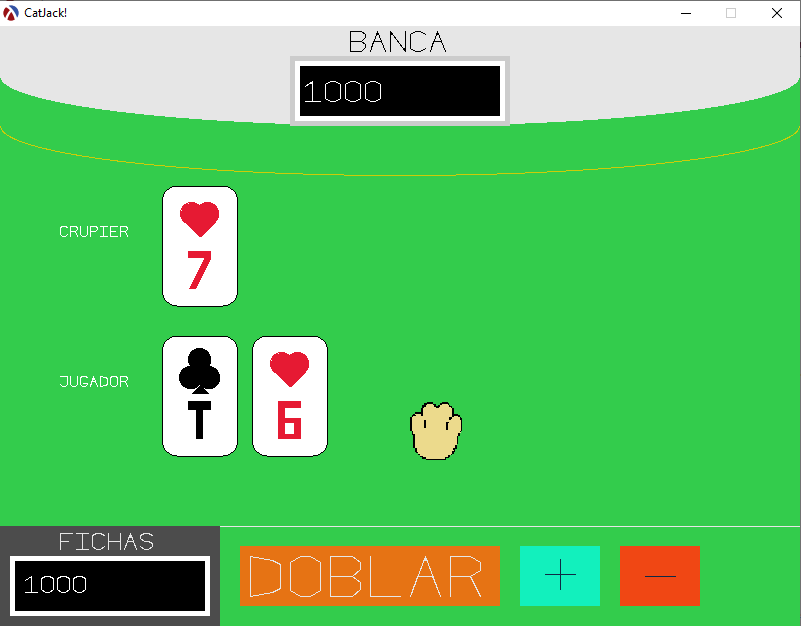
\includegraphics[width=0.5\linewidth]{img/mesa.png}
        \caption{Mesa de CatJack}
        \label{fig:enter-label}
    \end{figure}
\end{frame}

%------------------------------------------------
\subsection{Letras}
\begin{frame}{Letras}
La librería \textbf{\textit{graphics}} implementa impresión de cadenas, pero con poca \textbf{adaptabilidad}.
    \begin{itemize}
        \item \textbf{Solución}: implementar una tipografía completamente \textbf{manejable}.\\
    \end{itemize}
    
    Implementación compuesta por
    \begin{itemize}
        \item \textbf{Mapas de puntos} de cada símbolo disponible ([0-9A-ZÑ.+-]).
        \item Funciones de \textbf{impresión de cadena} que permita adaptar tamaño, color y posición.
    \end{itemize}
    
\end{frame}

%------------------------------------------------
\subsection{Juego}
\begin{frame}{Juego}
    El juego es \textbf{Point and click} (mecánica basada en ratón).\\
    El elemento básico del juego es el \textbf{botón}.\\
    \begin{itemize}
        \item Problema: \textbf{\textit{graphics}} no implementa botones.
        \item \textbf{Solución}: capturar clics y evaluar coordenadas de impacto.
        \begin{itemize}
            \item \textbf{Botones circulares}: región delimitada por distancia euclidiana.
            \item \textbf{Botones rectangulares}: región delimitada por coordenadas.
        \end{itemize}
    \end{itemize} 
\end{frame}

%------------------------------------------------
\begin{frame}{Juego (2)}
    Funcionalidades del juego:
    \begin{itemize}
        \item \textbf{Mazo}: se implementa un mazo de $52 \times 4$ cartas (usando listas) y la función de mezclar baraja.
        \item \textbf{Fichas iniciales}: se determinan las mismas para el \textbf{jugador} y para el \textbf{crupier}.    
        \item \textbf{TDAs}:
        \begin{itemize}
            \item \textbf{Jugada}: compuesto por la \textit{mano, fichas disponibles} y \textit{apuesta realizada}.
            \item \textbf{Ronda}: compuesto por \textit{ganador, mazo, fichas del jugador y fichas del crupier}.
        \end{itemize}
        \item \textbf{Reparto inicial}: se reparten dos cartas al jugador y una al crupier.
        \item \textbf{Determinar apuesta}: se determina la apuesta a realizar.
    \end{itemize}
\end{frame}
%------------------------------------------------
\begin{frame}{Juego (3)}
\begin{itemize}
    \item \textbf{Turno jugador}: opciones del jugador.
    \item \textbf{Turno del crupier}: saca cartas hasta tener una mano igual o mayor a 17.
    \item \textbf{Ronda}: se integra el reparto inicial, el turno del jugador, el turno del crupier y el resultado. Los \textbf{contadores} muestran fichas o rondas ganadas según el \textbf{modo de juego}. 
    \item \textbf{Blackjack}: se implementa el juego en dos funciones distintas:
    \begin{itemize}
        \item \textbf{blackjack-fichas}
        \item \textbf{blackjack-ganar}
    \end{itemize}
\end{itemize}
\end{frame} 
\section{Resultados} 

\begin{frame}{Carátula}
    \begin{figure}
        \centering
        
\includegraphics[width=0.6\linewidth]{img/caratula.png}
        \caption{Carátula del juego}
        \label{fig:caratula}
    \end{figure}
\end{frame}

\begin{frame}{Menús}
    \begin{figure}
        \centering
        
\includegraphics[width=0.6\linewidth]{img/menú_principal.png}
        \caption{Menú principal}
        \label{fig:principal}
    \end{figure}
\end{frame}

\begin{frame}{Menú rondas}
    \begin{figure}
        \centering
        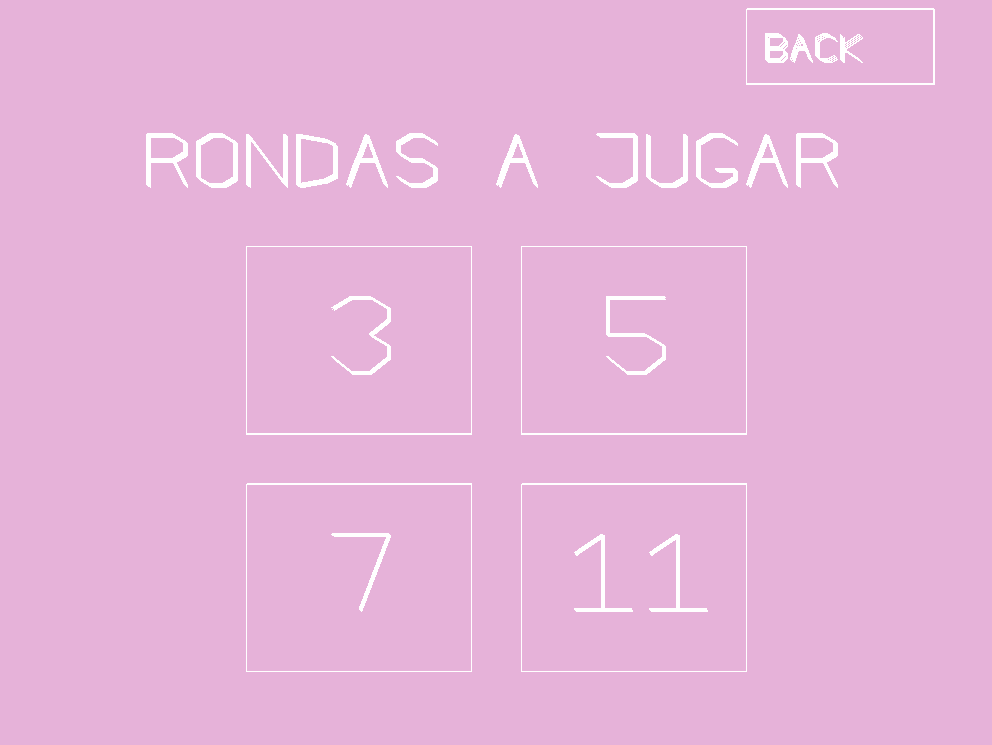
\includegraphics[width=0.6\linewidth]{img/menu_rondas.png}
        \caption{Menú del modo rondas}
        \label{fig:rondas}
    \end{figure}
\end{frame}

\begin{frame}{Tablero rondas}
    \begin{figure}
        \centering
        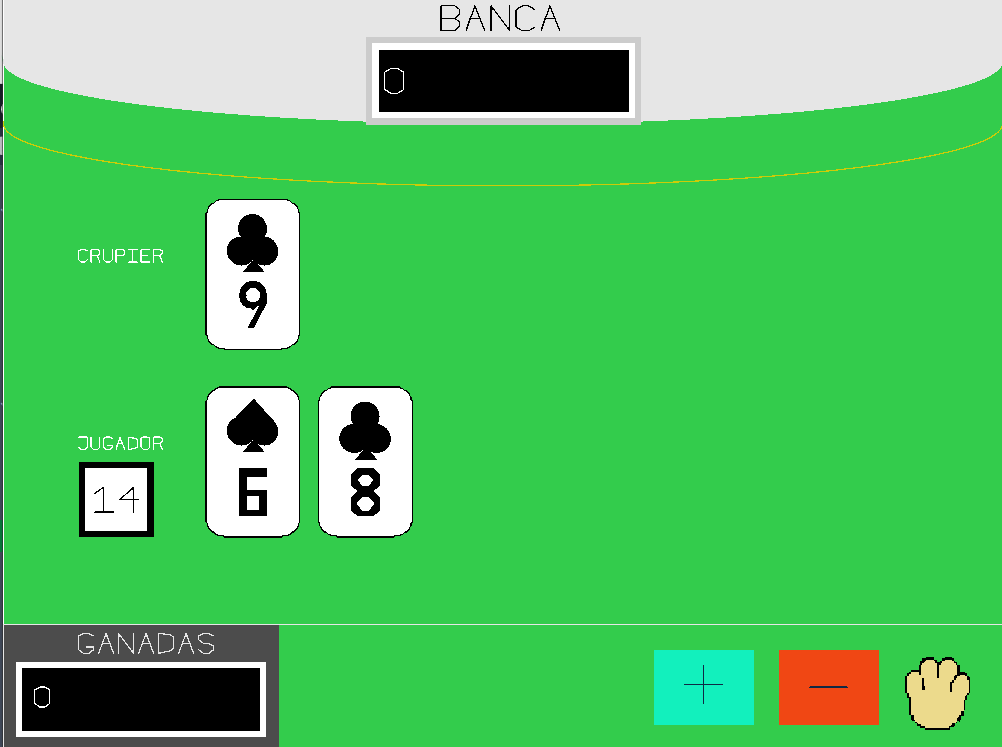
\includegraphics[width=0.6\linewidth]{img/tablero_rondas.png}
        \caption{Tablero del modo rondas}
        \label{fig:rondas-tablero}
    \end{figure}
\end{frame}

\begin{frame}{Mensaje de ganar ronda}
    \begin{figure}
        \centering
        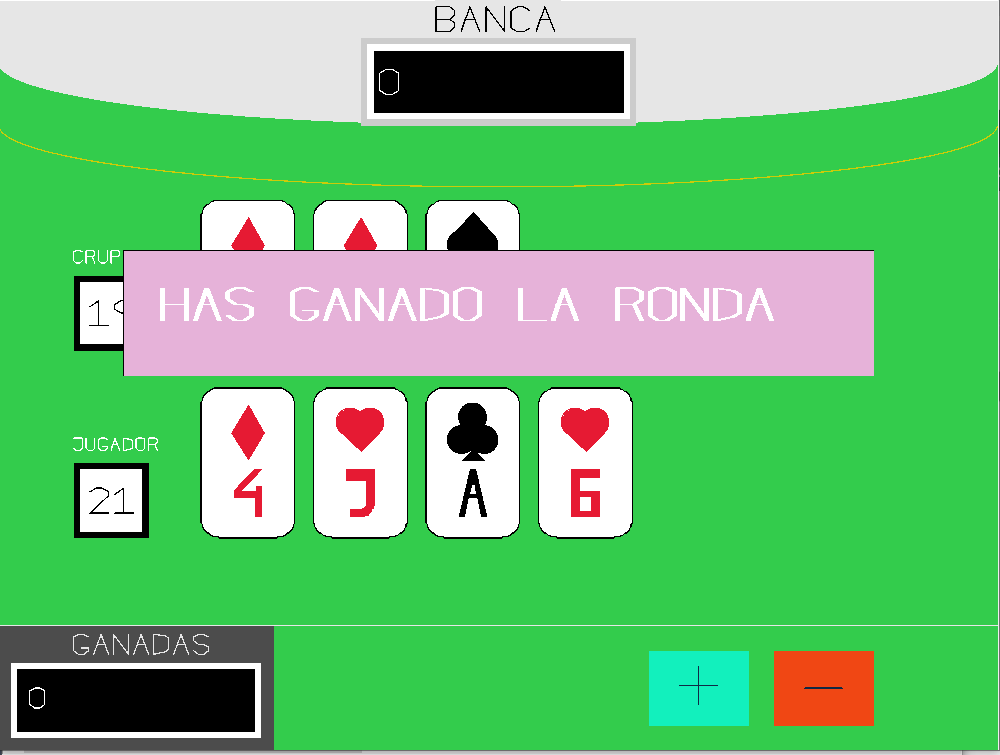
\includegraphics[width=0.6\linewidth]{img/ganar_ronda.png}
        \caption{Mensaje de ganar ronda (Jugador)}
        \label{fig:ganar_ronda}
    \end{figure}
\end{frame}

\begin{frame}{Mensaje de ganar ronda (2)}
    \begin{figure}
        \centering
        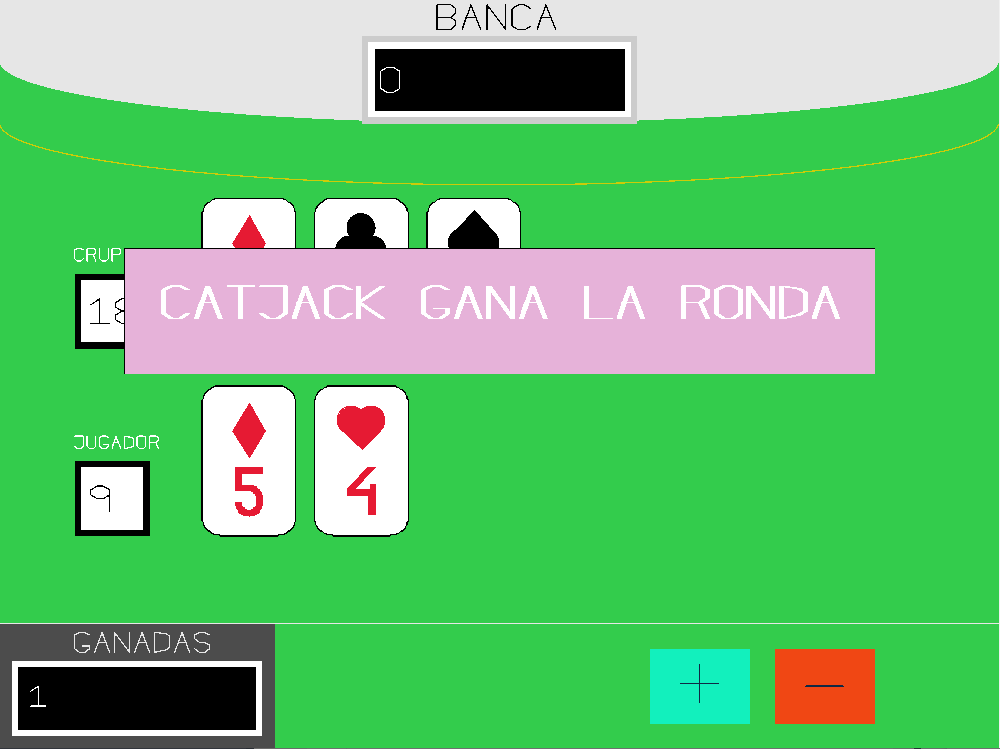
\includegraphics[width=0.6\linewidth]{img/ganar_ronda_c.png}
        \caption{Mensaje de ganar ronda (Crupier)}
        \label{fig:enter-label}
    \end{figure}
\end{frame}

\begin{frame}{Mensaje de ganar partida}
    \begin{figure}
        \centering
        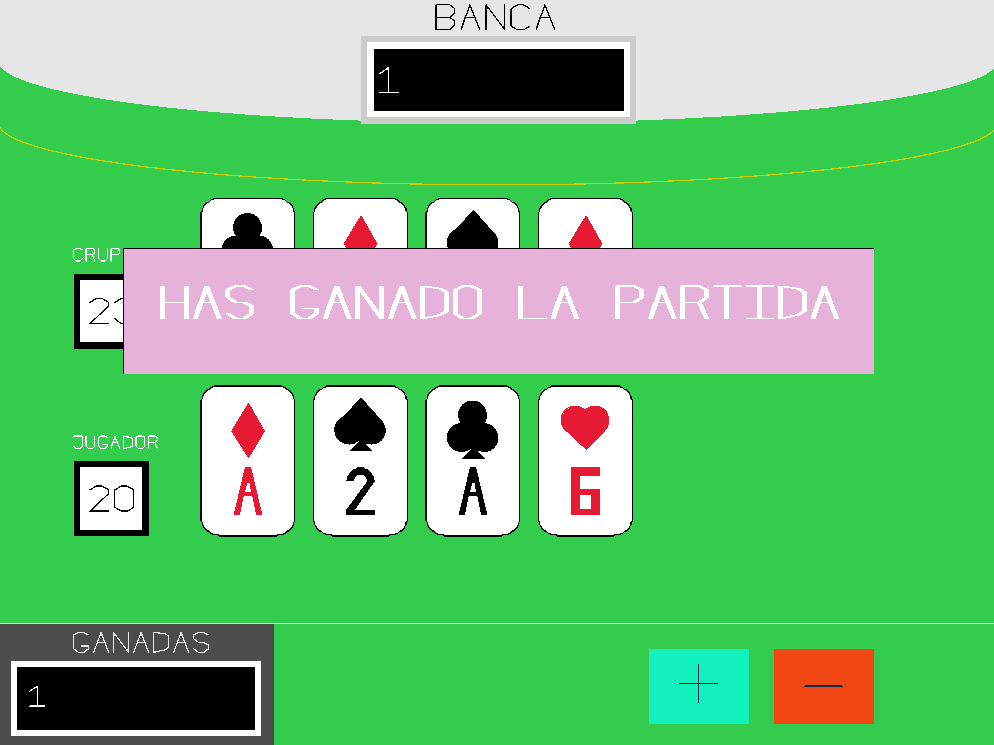
\includegraphics[width=0.6\linewidth]{img/mensaje_ganar.png}
        \caption{Mensaje de ganar partida (Jugador)}
        \label{fig:enter-label}
    \end{figure}
\end{frame}

\begin{frame}{Input fichas}
    \begin{figure}
        \centering
        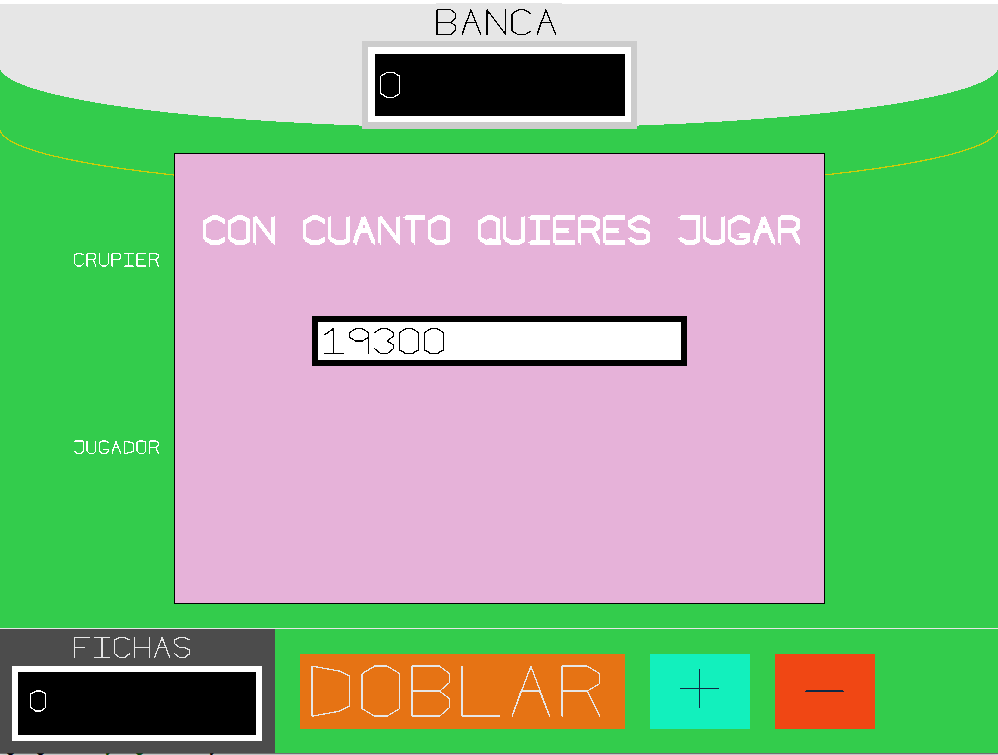
\includegraphics[width=0.6\linewidth]{img/input-fichas.png}
        \caption{Menú de input de fichas a jugar}
        \label{fig:input-fichas}
    \end{figure}
\end{frame}

\begin{frame}{Elegir apuesta}
    \begin{figure}
        \centering
        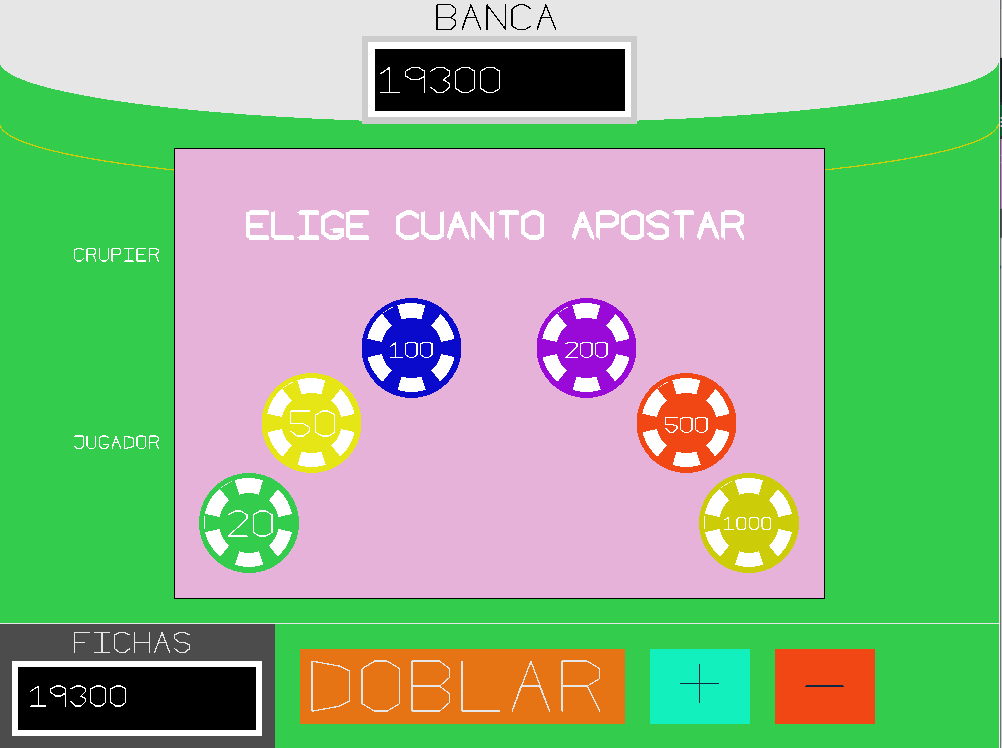
\includegraphics[width=0.6\linewidth]{img/elegir-apuesta.png}
        \caption{Menú de elección de apuesta de fichas}
        \label{fig:elegir-apuesta}
    \end{figure}
\end{frame}

\begin{frame}{Tablero fichas}
    \begin{figure}
        \centering
        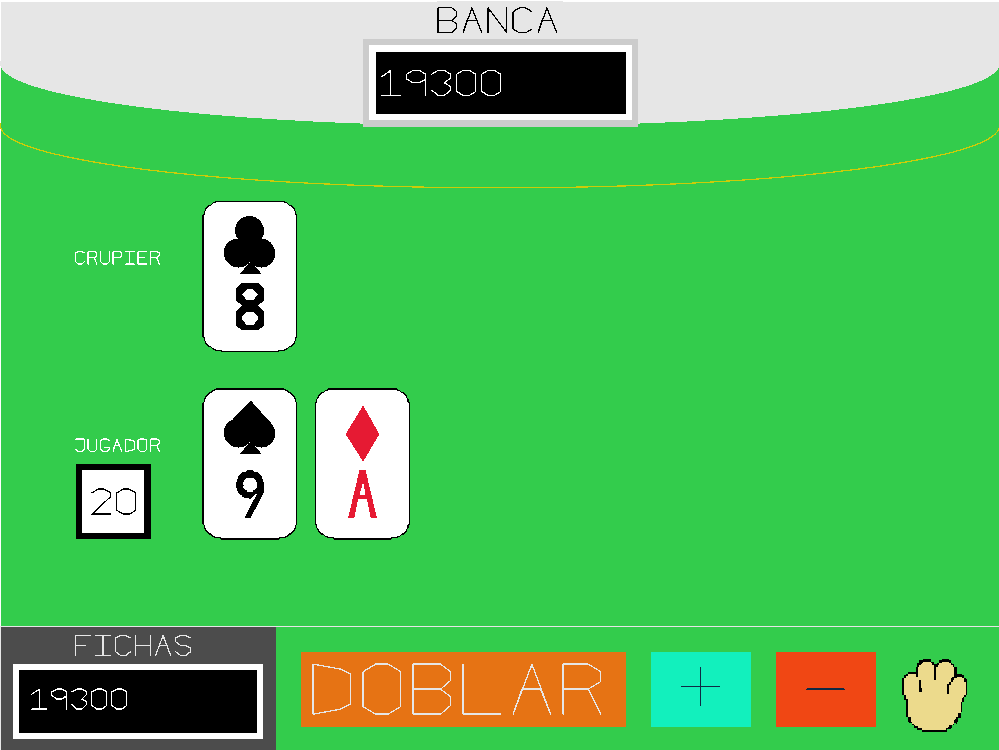
\includegraphics[width=0.6\linewidth]{img/tablero-fichas.png}
        \caption{Tablero de modo de juego fichas}
        \label{fig:fichas-tablero}
    \end{figure}
\end{frame} 
\section{Conclusiones}

\begin{frame}{Conclusiones}
    \begin{itemize}
        \item Los avisos de \textbf{doblar apuesta} no implementados: se muestra por \textbf{consola}.
        \item \textbf{Fluidez} de mis animaciones es mejorable (lenguaje interpretado). 
         \item La programación declarativa \textbf{destaca} por la fácil implementación que implica.
        \item Sin embargo, el \textbf{diseño modular} es complicado.
        \begin{itemize}
            \item Tipo de dato abstracto \textbf{no tan eficiente}.
            \item \textbf{Definir} y \textbf{redefinir} variables es \textbf{farragoso}.
        \end{itemize}
    \end{itemize}
\end{frame}

\begin{frame}
    \begin{itemize}
        \item Utilizar \textbf{graphics} ha supuesto un reto.
            \begin{itemize}
                \item Gran \textbf{personalización}.
                \item Ha requerido \textbf{mayor implementación}.
            \end{itemize}
        \item Librería con potencial \textbf{didáctico} para el desarrollo de motores gráficos.
        \item Ocasión para el desarrollo de mis competencias relacionadas con el diseño gráfico de \textbf{videojuegos 2D}.
    \end{itemize}
        
    
\end{frame} 
\section{Referencias}

\begin{frame}
    \begin{itemize}
        \item Racket Documentation. (2024, diciembre 16). \textbf{Racket documentation}. \href{https://docs.racket-lang.org/}{https://docs.racket-lang.org/}
        \item Wikipedia. (2024, diciembre 16). \textbf{Blackjack}. Wikipedia. \href{https://es.wikipedia.org/wiki/Blackjack}{https://es.wikipedia.org/wiki/Blackjack}
        \item Wikipedia. (2024, diciembre 16). \textbf{Rectas tangentes a circunferencias}. Wikipedia. \href{https://es.wikipedia.org/wiki/Rectas_tangentes_a_circunferencias}{https://es.wikipedia.org/wiki/Rectas\_tangentes\_a\_circunferencias}
        \item Pygame. (2024, diciembre 16). \textbf{Pygame}. \href{https://www.pygame.org/}{https://www.pygame.org/}
        \item GeoGebra. (2024, diciembre 16). \textbf{GeoGebra Classic}. \href{https://www.geogebra.org/classic}{https://www.geogebra.org/classic}
    \end{itemize}
\end{frame} 

%------------------
%	DIAPOSITIVA DE CIERRE
%------------------

\begin{frame}
	\begin{center}
		{\Huge ¡Gracias por su atención!}
	\end{center}
\end{frame}

%------------------

\end{document}
